\section{Kernel architecture}\label{sec:arch}

\subsection{Pauli frame sampling}\label{sec:frame-sampling}

A Pauli frame assigns to every qubit $q$ and shot a pair of bits $(x_q, z_q)$, the X and Z components of the Pauli
operator by which the noisy shot differs from the noiseless reference. Clifford gates map Pauli operators to Pauli
operators, so the frame is updated by fixed bit rules: H swaps $x_q$ and $z_q$, S sets $z_q \leftarrow z_q \oplus
x_q$, and CX with control $a$ and target $b$ sets $x_b \leftarrow x_b \oplus x_a$ and $z_a \leftarrow z_a \oplus z_b$.
A reset clears the frame of its qubit. A noise channel XORs a random Pauli into the frame. A measurement in the Z basis
flips the shot's outcome relative to the reference exactly when $x_q = 1$, and the analogous rules hold in the X basis
($z_q$) and the Y basis ($x_q \oplus z_q$). A detector is the parity of a set of measurement outcomes whose noiseless
parity is fixed, and the reference parity cancels when two shots are compared; the value of a detector in a shot is
therefore the XOR of the frame flips of its measurements. The kernel never needs the reference sample itself: it emits,
for each detector and logical observable, whether the shot deviates from the noiseless value. This is the quantity
Stim's detector sampler returns~\cite{gidney2021stim}.

With $L$ shots processed together, every frame component of a qubit is an $L$ bit word and every rule above is one
word wide bitwise operation. The kernel uses $L=\NumLanes$ lanes per instance.

\subsection{The first kernel and its costs}\label{sec:first}

The first kernel, built earlier in this project and not published, interprets a stream of instructions one at a
time. Each step fetches a 41 byte
instruction from HBM, applies it to a frame of 64 lanes, draws noise from a 64 lane Philox bank inside the same step,
and on every measurement runs a loop over all 256 detector accumulators to apply the detector mask of that
measurement. Its instruction loop was not pipelined (an attempt to pipeline it reached an initiation interval of 34
cycles and exceeded the resource budget), and each kernel launch sampled 64 shots. These costs, rather than any
property of the algorithm, set its throughput: at a 250~MHz kernel clock it sampled the benchmark circuits of
Section~\ref{sec:setup} at \NumFirstKernelRep{}, \NumFirstKernelSurfThree{} and \NumFirstKernelSurfFive{} shots per
second on one card, below one Stim process on an AMD EPYC 7742. Its output was nevertheless correct: on hardware its
detector rates and its decoded logical error rates (up to distance 5) agreed with Stim, and single fault injection
reproduced all \NumFirstTierThreeTotal{} error mechanisms of the detector error models of three circuits. The kernel described next keeps the instruction semantics of the first
kernel and its software model, and changes how they are executed.

\subsection{Dataflow structure}\label{sec:dataflow}

Figure~\ref{fig:kernel} shows the kernel. At the start of a launch the program and the fold list are copied from HBM
into on chip memory once. Four stages then run concurrently, connected by FIFO streams, over all batches of the
launch:
\begin{enumerate}
\item the noise stage reads one slot per cycle and computes the noise masks of its instruction for all lanes;
\item the frame stage applies one slot per cycle to the Pauli frame and emits the frame flip of every
measurement;
\item the fold stage collects the measurement flips of a batch and computes every detector and observable as the XOR
of its listed measurements;
\item the store stage writes the outputs of every batch to HBM in bursts.
\end{enumerate}
Every loop of every stage is pipelined with an initiation interval of one cycle. The frame stage needs exactly one
cycle per slot, and the other stages need fewer cycles per batch than it does, so a batch of \NumLanes{} shots takes
as many cycles as its program has slots.

\begin{figure}[t]
\centering
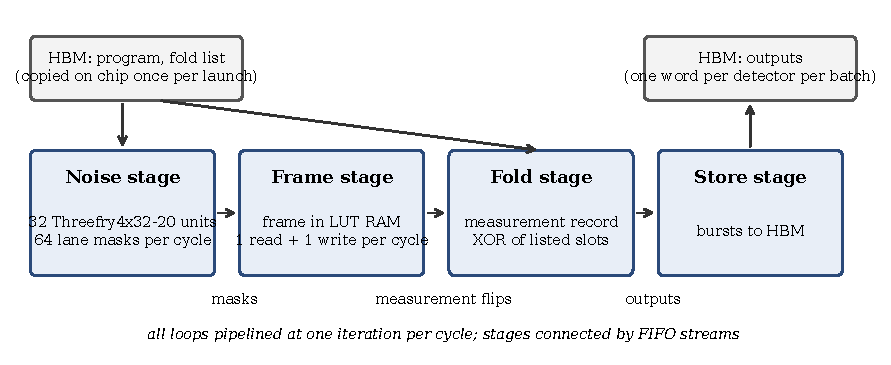
\includegraphics[width=\textwidth]{figures/fig_kernel.pdf}
\caption{Dataflow structure of one kernel instance. The noise stage evaluates \NumPairs{} Threefry4x32-20 units
per cycle; the frame stage keeps the frames in a one read, one write memory and completes every slot two cycles after its
read; the
fold stage keeps a per batch record of measurement flips. Stages are connected by FIFO streams and work on different
instructions or batches at the same time.}\label{fig:kernel}
\end{figure}

\subsection{Program and compiler}\label{sec:program}

The compiler takes a Stim circuit and produces the same instruction list as for the first kernel: broadcast
instructions are split into one instruction per qubit or qubit pair, REPEAT blocks are unrolled, and the measurement
records that every DETECTOR and OBSERVABLE\_INCLUDE refers to are resolved to absolute measurement indices. It then
applies three transformations specific to this kernel. First, qubits are renumbered densely in order of first use:
the generated surface code circuits use sparse qubit indices, and dense numbering lets a distance 7 surface code
(\NumSlotsSevenQubits{} qubits) fit the \NumQubitsMax{} entries of the frame. Second, every measurement receives a slot in
the measurement record of a batch, and the detector and observable definitions become a fold list: for every output in
order, the record slots of its measurements, with the last entry of each output marked. Third, the instructions are
scheduled for the frame pipeline (Section~\ref{sec:frame}). Every slot is encoded in 64 bits: opcode, the 7 bit index of
the qubit it reads and writes, two flags marking the first and the second slot of a two qubit instruction, an 11 bit
record slot and the 32 bit noise threshold $\lfloor p\cdot 2^{32}\rceil$. Table~\ref{tab:programs} lists the compiled programs.

\subsection{Noise stage}\label{sec:noise}

The noise masks of an instruction depend only on the instruction, the lane and the batch, never on the frame. The noise
stage therefore runs ahead of the frame stage and is decoupled from it by a stream. It uses a counter based generator
from the family of Salmon et al.~\cite{salmon2011random123}, whose members pass the TestU01 BigCrush battery: the output
is a fixed function of a 128 bit counter and a key, so the generator has no state to carry and any draw can be
recomputed in software. For an instruction whose (first) slot is $i$, lane $l$ and batch $g$ the stage evaluates
Threefry4x32-20 with counter $(i, \lfloor l/2\rfloor, g, 0)$ and the node's key. One evaluation yields four 32 bit
words; even lanes use the first two and odd lanes the last two, so \NumPairs{} generator units serve \NumLanes{} lanes
per cycle. For lane $l$ the first word $w_0$ decides whether the channel fires ($w_0 < t$ for the threshold $t$) and
the second word $w_1$ selects which Pauli: $w_1 \bmod 3$ for single qubit depolarizing noise and $w_1 \bmod 15$ for two
qubit depolarizing noise, as in the first kernel and its model. The modulo needs no divider: since $16 \equiv 1
\pmod{15}$, a 32 bit word and the sum of its eight hexadecimal digits are congruent modulo 15, the sum is at most 120,
and one more digit sum and a conditional subtraction give the exact residue; $w_1 \bmod 3$ follows from $w_1 \bmod
15$. The twenty Threefry rounds are pipelined, giving the stage a depth of \NumDepthNoise{} cycles at one slot per
cycle.

The first kernel used Philox4x32-10 from the same family, and so did the first versions of this
kernel. Philox multiplies two 32 bit words in each of its ten rounds; \NumPairs{} pipelined Philox units took
\NumPhiloxDsp{} DSP blocks per instance, \NumPhiloxDspSlr\,\% of those of one SLR. Threefry instead uses only
additions, rotations and exclusive ors, which map to ordinary logic and carry chains: an instance needs
\NumHlsDsp{} DSP blocks. Why this mattered is reported in Section~\ref{sec:res-impl}. The software model computes the
same Threefry function; it reproduces the known answer of the Random123 reference for counter and key zero and agrees
with the ThreeFry generator of the randomgen package on random counters and keys.

\subsection{Frame stage and hazard free scheduling}\label{sec:frame}

The frame stage must apply one instruction per cycle to a frame of up to \NumQubitsMax{} qubits, each with two words
of \NumLanes{} bits. We first held the frame in registers, so that a two qubit instruction could read both of its
qubits and write both back in one cycle. That version reached one instruction per cycle in synthesis after the read,
the gate logic and the write back were split into pipeline steps, but its implementation on the card failed: with two instances, the
routed design failed Vivado's verification with conflicting nets after more than five hours of implementation. A
congestion analysis of that design attributes the most congested short range windows to the frame stage, whose
register crossbar (four 128 way selections and write paths into all frame registers) is local and dense, and the
global and long range windows mostly to the noise stage, whose Philox multipliers fill the DSP columns of their
region. The kernel therefore keeps the frame in a small memory with one read
and one write per cycle, implemented in LUT RAM, and gives every slot exactly one frame read and one frame write. A
single qubit instruction occupies one slot. A two qubit instruction occupies two consecutive slots: the first reads
qubit $a$, the second reads qubit $b$, and their new values are written in the two following cycles. In each cycle
the stage reads the qubit of slot $k$ and completes slot $k-2$ from the operands read two and one cycles earlier; for
the first slot of a pair it computes the new values of both qubits, writes $a$ and keeps $b$, which the second slot
writes one cycle later. A valid bit per qubit, cleared at the start of each batch, makes an unwritten qubit read as
zero, so the memory never needs to be cleared. The synthesised frame loop runs at one slot per cycle with a depth of
\NumDepthFrame{} cycles, and the instance needs \NumHlsLutSlr\,\% of the LUTs of one SLR.

The price is a hazard: the result of slot $k$ is written at the end of cycle $k+2$, so a slot that reads a qubit
fewer than three slots after a slot that touched it sees a stale value. The frame stage does not detect this. Instead
the compiler guarantees that it never happens:

\begin{proposition}\label{prop:schedule}
If every two slots that touch a common qubit are at least $D \ge 3$ apart, the frame stage computes the same frame,
measurement flips and outputs as executing the instructions one at a time in slot order.
\end{proposition}

\begin{proof}
Slot $k$ reads its qubit in cycle $k$, and the value of slot $k'$ is written at the end of cycle $k'+2$, so the read
sees the result of every slot $k'\le k-3$ and of no later slot. Every earlier slot on the same qubit has $k'\le k-D\le
k-3$, so the value read is the one the sequential execution would read. For a pair occupying slots $k$ and $k+1$, the
new values are computed in cycle $k+2$ from the operands of both slots, which are correct by the same argument for
each of the two qubits. Slots on disjoint qubits do not interact, and the measurement flip of a slot is computed from
its correct operands.
\end{proof}

The compiler enforces $D=\NumHazardDistance$, more than the three slots needed, as margin for the cycle in which the
synthesised hardware performs the read and the write; RTL cosimulation of the repetition code, in which \NumRepReusesAtD{} of the \NumRepReuses{} reuses
of a qubit are at the minimum distance, confirms that the margin holds. The scheduler fills slots one by one: each slot, or pair of
slots, takes the earliest instruction in compiler order whose qubits were last touched at least $D$ slots before and
whose predecessors on each of its qubits are already placed, or a NOP if there is none. The order of the instructions
on every qubit is unchanged, and instructions on disjoint qubits commute, so the schedule computes the same frame as
the compiler order. The program begins and ends with $D$ NOPs, which write nothing, so that no write or measurement of
one batch reaches past the clear of the valid bits at the start of the next. Two qubit instructions cost two slots,
and NOPs cost slots only when a circuit has too little parallelism: Table~\ref{tab:programs} shows
\NumNopsSurfFive{} NOPs, all of them padding, for the distance 5 surface code, and more for the small repetition
code, whose five qubits cannot fill the slots between reuses.

The scheduler is checked by tests that every two slots on a qubit are at least $D$ apart, that the two slots of a
pair are consecutive, that the program begins and ends with $D$ NOPs, and that the sequence of instructions on every
qubit is identical to the compiler order. A negative control shows that the C simulation of the kernel models the
delayed write: compiled with $D=2$, a circuit whose every instruction depends on the one before produces output that
differs from the software model.

\subsection{Fold and store stages}\label{sec:fold}

The first kernel folded each measurement into the detectors immediately, which needs a read, modify and write of
detector accumulators that two nearby measurements may share. Here the frame stage only sends the flip of every
measurement, tagged with its record slot, to the fold stage, which writes it into a measurement record of the batch.
When all measurements of the batch have arrived, the fold stage walks the fold list once, XORing the record entries
of each output into an accumulator that is emitted at the last entry. The accumulator is the only state carried from
one entry to the next, and the loop runs at one entry per cycle. The fold of batch $g$ overlaps the frame simulation
of batch $g+1$, which needs a FIFO deep enough to hold the measurement flips produced meanwhile. The store stage
writes the outputs of every batch to HBM in bursts: for each batch, one word of \NumLanes{} bits per detector and per
observable, bit $l$ belonging to shot $l$ of the batch.

\subsection{Several instances per card}\label{sec:instances}

The Alveo U55C device has three super logic regions (SLRs); SLR0 also holds the platform's HBM controllers and DMA
engine. A card holds \NumInstancesPerCard{} instances of \NumLanes{} lanes, placed in SLR1 and SLR2 and connected to
their own HBM pseudo channels through the SLR crossings. The
instances of a card run independently, on disjoint batch ranges (Section~\ref{sec:nodes}).
